\begin{figure}[!htb]
  \centering
  \begin{subfigure}{0.33\textwidth}
    \centering
    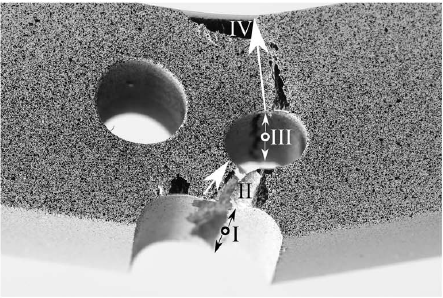
\includegraphics[width=\textwidth,scale=0.5]{Chapter5/figures/3pb/1234}
    \caption{experiment}
    \label{fig: Chapter5/3pb/1234/experiment}
  \end{subfigure}
  \hfill
  \begin{minipage}{0.6\textwidth}
    \begin{subfigure}{0.45\textwidth}
      \centering
      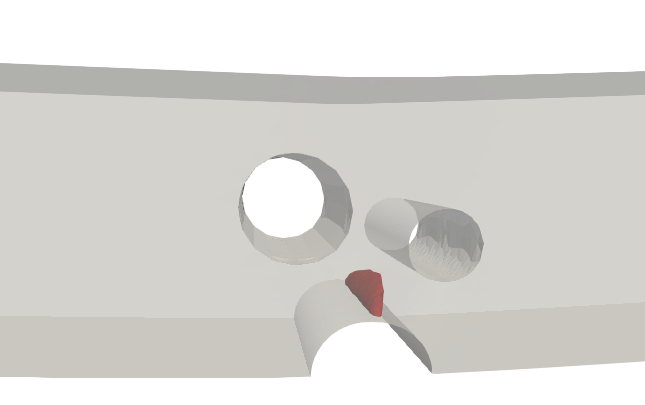
\includegraphics[width=\linewidth]{Chapter5/figures/3pb/I}
      \caption{stage I}
      \label{fig: Chapter5/3pb/1234/simulation_I}
    \end{subfigure}
    \begin{subfigure}{0.45\textwidth}
      \centering
      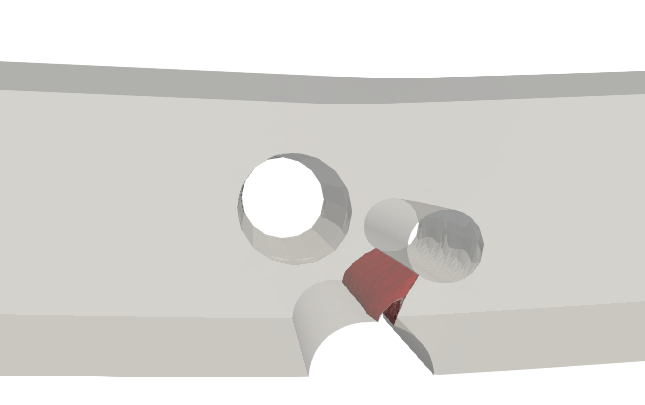
\includegraphics[width=\linewidth]{Chapter5/figures/3pb/II}
      \caption{stage II}
      \label{fig: Chapter5/3pb/1234/simulation_II}
    \end{subfigure}
    
    \begin{subfigure}{0.45\textwidth}
      \centering
      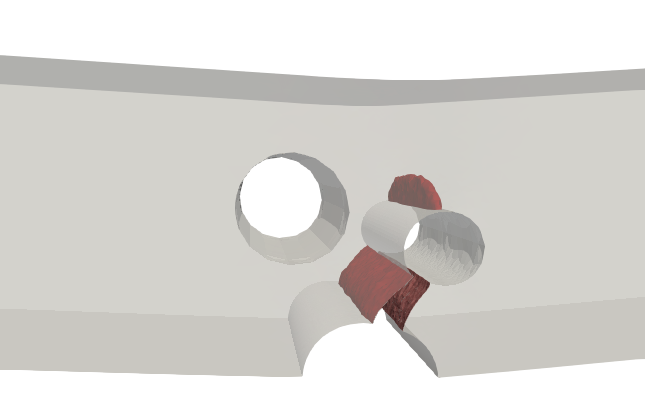
\includegraphics[width=\linewidth]{Chapter5/figures/3pb/III}
      \caption{stage III}
      \label{fig: Chapter5/3pb/1234/simulation_III}
    \end{subfigure}
    \begin{subfigure}{0.45\textwidth}
      \centering
      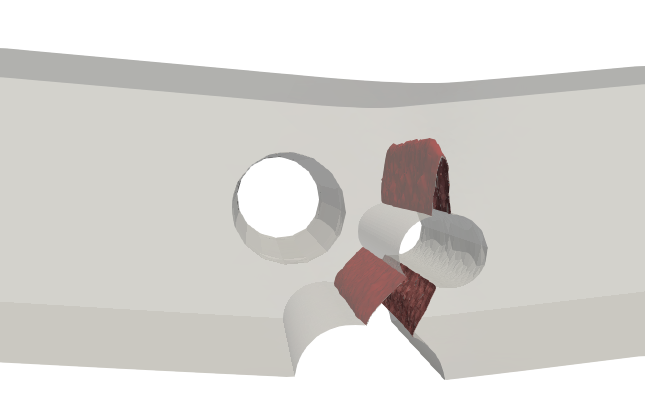
\includegraphics[width=\linewidth]{Chapter5/figures/3pb/IV}
      \caption{stage IV}
      \label{fig: Chapter5/3pb/1234/simulation_IV}
    \end{subfigure}
  \end{minipage}
  \caption{Comparison of crack paths between (a) the experiment \cite{kubik2019ductile} and (b-e) the simulation with $\beta = 0.1$ and $\varepsilon_0 = 0.2$. Iso-contours of $d=0.8$ are highlighted in red. }
  \label{fig: Chapter5/3pb/1234}
\end{figure}
